\section{Application of Trade-Off Model}

By calculating our two scores, ecological and economic, we can apply our impact score calculations to virtually any invasive species. For the purposes of our discussion, our choice of three commonly-regarded-to-as invasive or foreign plants species from the United States region includes: \textit{dandelions} in New York, \textit{garlic mustard plants} in Illinois, and  \textit{English ivy} plants in Washington \cite{columbiatribuneDandelionsFight, natureGarlicMustard, invasiveEnglishHedera}.

[background on dandelion, garlic mustard, and English ivy plants]

\subsection{Dandelion Plants}
\subsubsection{Ecological Impact Score}

To first determine the ecological impact score of dandelion plants, we examine the top 3 closely-related native species where dandelions reside in New York, which include the following species.

\begin{itemize}
    \item \textbf{Bombus impatiens} (Bumblebees) — native pollinators common to eastern North America that commonly visit dandelion species to obtain pollen and help dandelions reproduce, therefore, they have a mutualistic relationship \cite{nwfCommonEastern}.
    \item \textbf{Malacosoma americanum} (Moths) — feeds on the leaves of the common dandelion in New York. A consumer-plant relationship with dandelions \cite{butterfliesandmothsEasternTent}.
    \item \textbf{Cuscuta gronovii} (Scaldweed) — a climbing parasitic vine that extracts nutrients from attached-to plants \cite{minnesotawildflowersCuscutaGronovii}.
\end{itemize}

Below, we determined an interaction matrix for the Lotka-Volterra model based on the interactions of each species in row \(i\) to the species in column \(j\). Therefore, each \(\alpha_{ij}\) represents the interaction of species \(j\) on species \(i\). For example, if species \(j\) was a natural predator of species \(i\), the value of \(\alpha_{ij}\) will be a negative value. If two species were mutualistic, we would expect that the element \(\alpha_{ij}\) would be indeed positive, thus improving the rate of growth of either population. Note that generally, element \(\alpha_{ij} \neq \alpha_{ji}\) because the effect species \(i\) has on species \(j\) is generally opposite to the effect in the reverse order. Furthermore, the impact of the invasive species on native populations is found in the fourth row and column of matrix \(\alpha\).

Assuming a starting population each of 100 plant units and a carrying capacity of 1000 plant units each, and growth rate of 0.005 for bumblebees, as their populations mostly fluctuate by seasons, 0.06 for moths as their populations grow quickly, 0.01 for vines as their populations tend to stabilize, and 0.04 for dandelions as show in the following logistic regression section \cite{nwfCommonEastern, butterfliesandmothsEasternTent, minnesotawildflowersCuscutaGronovii}. We solve the systems of differential equations show in Equation~\ref{eq:lotkavolterra} with the following interaction matrix approximated based on the relationships between each species.

\begin{equation}
        \alpha_{\text{ dandelion}} = {\underbrace{\begin{bNiceMatrix}[first-row,first-col]
        &&&&& \\
    \text{Bumblebees} && 1 & 0.25 & -0.5 & 2 &\\
    \text{Moths} && 0.25 & 1 & 0.6 & 0 &\\
    \text{Vines} && -0.5 & -0.5 & 1 & 2 &\\
    \text{Dandelions} && 2 & 0.25 & -1 & 1 & \\
    \end{bNiceMatrix}}_{ \\ \text{3 native species, 1 invasive species}}}
\end{equation}

From graphing the population solutions to the system, we can see the population shifts in Figure~\ref{fig:lotkavolterradandelion}. Based on the numerical solution to this differential equation from scientific computing software, we find the change of populations over a single year (365 days) to be \(\frac{1200}{100}\) for moths, \(\frac{250}{850}\) for vines, and \(\frac{550}{100}\) for bumblebees. So, we can calculate the native species impact score to be

\[\chi = \frac{1200}{100} + \frac{250}{850} + \frac{550}{100} = 17.794\]
%% need to do some graphing and calculations

\begin{figure}[h!]
\centering
    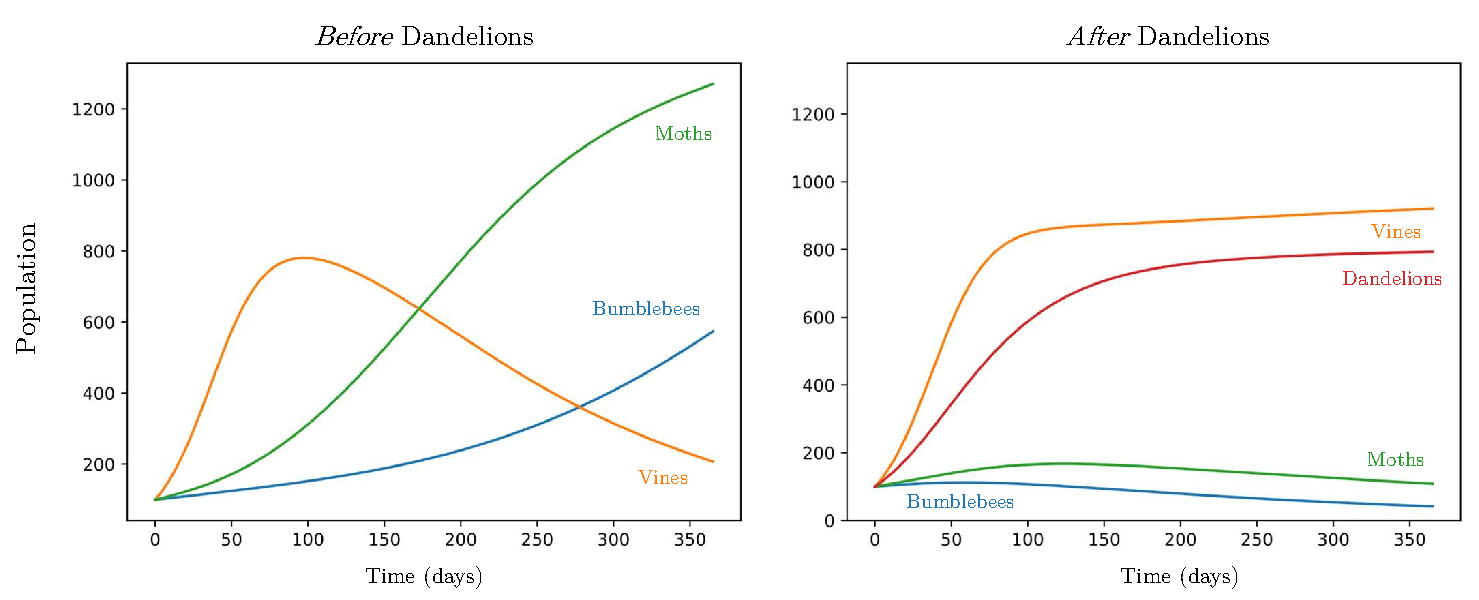
\includegraphics[scale=0.5]{figures/lotkavolterradandelions.pdf}
    \captionsetup{width=0.9\textwidth}
    \caption{\textbf{Before and after plot of native species populations of introduction of dandelion species}. Based on Lotka-Volterra competitor system of differential equations.}
    \label{fig:lotkavolterradandelion}
\end{figure}

Next, we calculate the spreadability index by performing logistic regression on dandelion data from the previous model. From plant population predictions in New York, we find that the carrying capacity of a region is approximately 900 dandelion plants, with a relatively logistic-shaped curve. Therefore, we calculate from logistic regression and finding the best-fit logistic curve, that the spreadability score (or proportionality of growth) is \(r = 0.04\), therefore our spreadability score is \(100r = 4\).

By Equation~\ref{eq:ecologicalimpact}, we see that our total ecological impact score is \(4 + \chi = 4 + 17.794 = 21.794\).

\subsubsection{Economic Potential}

To estimate economic profits, we assume there exists some small dandelion harvesting firm in New York. So, we proceed with analyzing the microeconomics of the business.

According to a variety of sources, we can approximate the marginal cost of harvesting each dandelion to be around \(\$0.10\) per unit of effort (to harvest one pound of dandelions) \cite{farmshowGrowingDandelions, gardeningknowhowDandelionHarvest}. We can approximate the marginal revenue curve by utilizing the fact that marginal revenue decreases for every five pounds of dandelions sold with maximum marginal revenue at around \(\$4.50\) per pound of dandelions \cite{farmfitlivingMakeMoney}. So, we can model marginal revenue with a linear model with slope -0.2 and y-intercept 4.5. From integration, we can calculate the the total revenue and total cost curve based on effort levels, which is shown in Figure~\ref{fig:dandelionprofits}. Therefore, we calculate dandelion profits (\(\pi_{\text{dandelions}}\)) be around \(\$47.86\).

\begin{figure}[h!]
\centering
    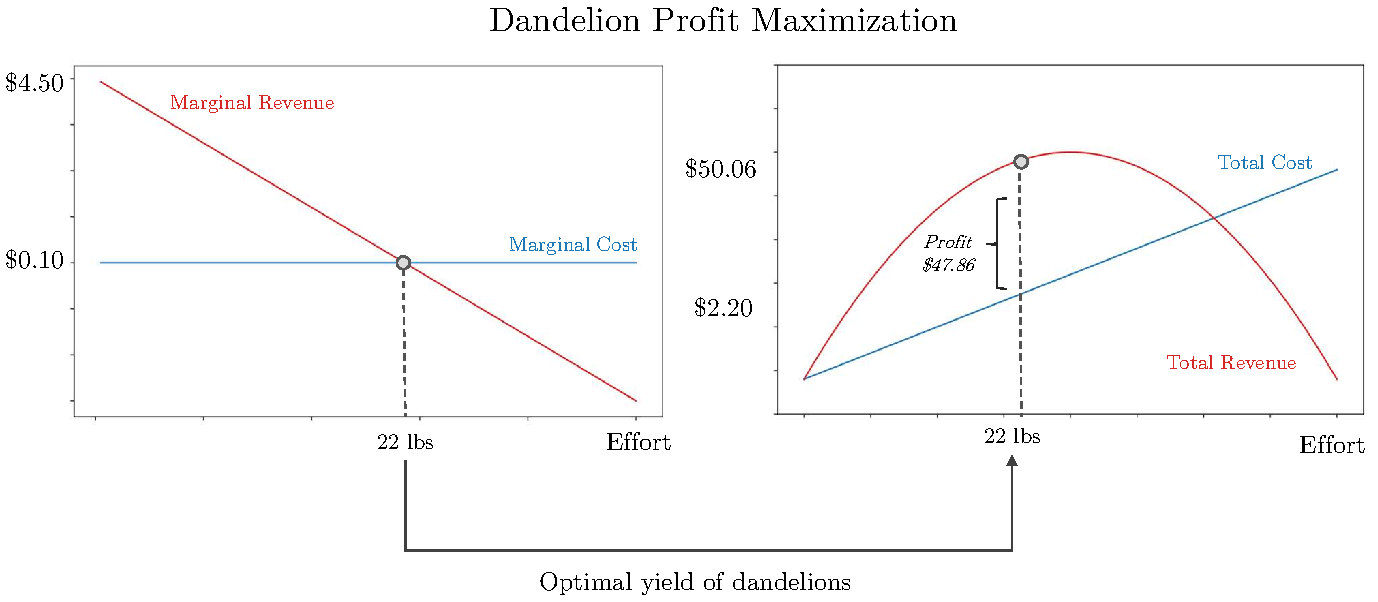
\includegraphics[scale=0.5]{figures/dandelionprofitmax.pdf}
    \captionsetup{width=0.9\textwidth}
    \caption{\textbf{Gordon-Schaefer model for dandelion profit yield.}}
    \label{fig:dandelionprofits}
\end{figure}

On top of calculating potential economic profits of a small dandelion business in New York, we additionally need to calculate the social welfare benefits and potential human risks. The average population of a New York town , is approximately \(n = 60,000\), and the net external benefit for each individual is approximately \(\$0.002\) as a rarely used medicinal plant and common soil loosener which can improve the growth of other harvested plants \cite{healthlineDandelionHealth}. Furthermore, for the New York, the Gini coefficient is 0.52 \cite{statistaBetweenRich}. Therefore, the social welfare output is \[W = (1- 0.52) \sum_{i = 1}^{60000} 0.002 = \$57.60\].

As a final part of calculating potential economic profits, we find the human health risk by calculating the amount of harm of a dandelion has on its surrounding human population. Since the only potential harm a dandelion could impose would be to people with dandelion allergies, we deduce that the potential human risk would be \(R = 0\).

With the three components of the economic potential score, we can calculate the score to be 

\[\text{Total Economic Benefit } = \pi + W - R = 47.86 + 57.60 - 0 = \$105.46\]

So, our final invasive species impact score is

\[\text{Impact Score} = (\text{Ecological Score, Economic Score}) = (21.794, \$105.46)\]

\subsection{Garlic Mustard Plants}

\subsubsection{Ecological Impact Score}

Next, to determine the ecological impact score of garlic mustard plants, we examine the top 3 closely-related native species where garlic mustard plants reside in Illinois, which include the following species.

\begin{itemize}
    \item \textbf{White trillium} (Wildflower) — native wildflower that grow in woodlands often threatened by garlic mustard invasion \cite{usdaGreatWhite}.
    \item \textbf{Plethodon cinerus} (Salamander) — amphibian that lives under leaves and forests and feeds on insects and other small inveterbrates \cite{amphibiawebAmphibiaWebPlethodon}.
    \item \textbf{Hylocichla mustelina} (Wood thush) — a songbird that nests in forests where garlic mustard invasion reduces vegetation for nesting cover \cite{allaboutbirdsWoodThrush}.
\end{itemize}

% https://extension.illinois.edu/invasives/garlic-mustard

Below, we again determined an interaction matrix for the Lotka-Volterra model based on the interactions of each species in row \(i\) to the species in column \(j\). Note that we again assume that the starting population of each species is units with a carrying capacity of 1000 plant units each, and a growth rate of 0.06 for wildflowers, as their populations mostly fluctuate by seasons, 0.03 for salamanders as their populations do not grow as quickly, 0.01 for songbirds as their populations tend to stabilize, and 0.1 for garlic mustard plants as their populations tend to grow very quickly. We solve the systems of differential equations show in Equation~\ref{eq:lotkavolterra} with the following interaction matrix approximated based on the relationships between each species.

\begin{equation}
        \alpha_{\text{ garlic mustard}} = {\underbrace{\begin{bNiceMatrix}[first-row,first-col]
        &&&&& \\
    \text{Wildflower} && 1 & 0.75 & 1.5 & -1 &\\
    \text{Salamanders} && 0.35 & 1 & 0.65 & -1 &\\
    \text{Songbirds} && 0.5 & 0.5 & 1 & -1 &\\
    \text{Garlic mustard} && 0.25 & 0.25 & 0.15 & 1 &\\
    \end{bNiceMatrix}}_{ \\ \text{3 native species, 1 invasive species}}}
\end{equation}

In the fourth column, since garlic mustard plants have a negative impact on all three of the native species populations, we assigned a value of -1 to each element. 

From graphing the population solutions to the system, we can see the population shifts in Figure~\ref{fig:lotkavolterragarlicmustard}. Based on the numerical solution to this differential equation from scientific computing software, we find the change of populations over a single year (365 days) to be \(\frac{100}{100}\) for wildflowers, \(\frac{800}{400}\) for salamanders, and \(\frac{400}{200}\) for songbirds. So, we can calculate the native species impact score to be

\[\chi = \frac{150}{100} + \frac{800}{450} + \frac{400}{200} = 5.278\]
%% need to do some graphing and calculations

\begin{figure}[h!]
\centering
    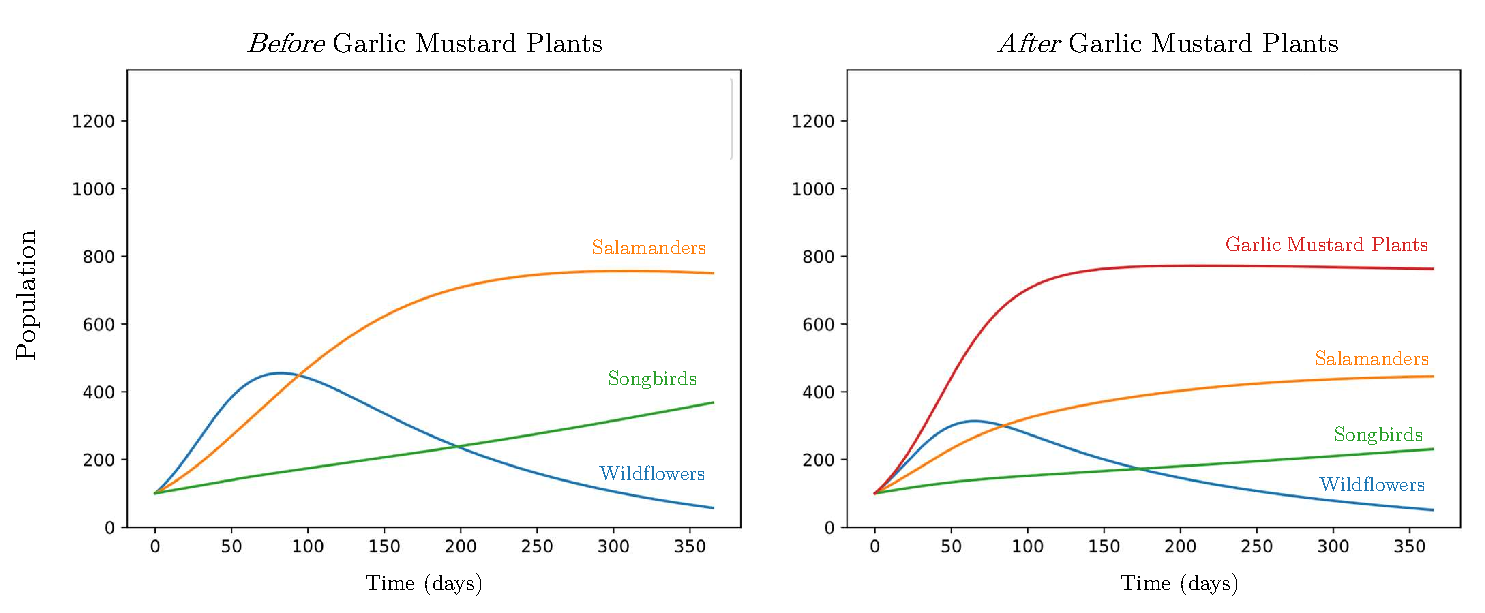
\includegraphics[scale=0.5]{figures/lotkavolterragarlicmustard.pdf}
    \captionsetup{width=0.9\textwidth}
    \caption{\textbf{Before and after plot of native species populations of introduction of Garlic mustard species}. Based on Lotka-Volterra competitor system of differential equations.}
    \label{fig:lotkavolterragarlicmustard}
\end{figure}

To calculate the spreadability index, we can start from a commonly regarded fact that Garlic mustard populations can double in a year in most growing conditions \cite{fmrInvasiveSpecies}. Therefore, by performing logistic regression with the x-axis being days and the y-axis as population, we can find that the \(r\) value is around 0.05. So, our spreadability index can be calculated as \(100r = 5\). Therefore, by Equation~\ref{eq:ecologicalimpact}, our ecological impact score is \(5 + \chi = 5 + 5.278 = 10.278\).

\subsubsection{Economic Potential}

As harvesting efforts for garlic mustard plants are minimal-to-none, we conclude that there is no possibility of a garlic mustard harvesting farm. This means that there is \textit{no potential economic profit} in a plot of land for a garlic mustard growth. Therefore, our economic profit \(\pi = 0\).

We additionally need to calculate the social welfare benefits and potential human risks of Garlic mustard plants. The population of an average town in Illinois, is approximately \(n = 50,000\), and the net external benefit for each individual is similar to dandelions at approximately \(\$0.002\) as a rarely used medicinal plant and herb \cite{fmrInvasiveSpecies}. Furthermore, for the Illinois, the Gini coefficient is 0.48 \cite{247wallstIncomeInequality}. Therefore, the social welfare output is \[W = (1- 0.48) \sum_{i = 1}^{50000} 0.001 = \$26.00\].

As a final part of calculating potential economic profits, we find the human health risk by calculating the amount of harm of population of garlic mustard plants has on its surrounding human population. Since garlic mustard plants are edible, the only potential harm a dandelion could impose would be to people with garlic mustard plant allergies, so we deduce that the potential human risk would be \(R = 0\) \cite{fmrInvasiveSpecies}.

With the three components of the economic potential score, we can calculate the score to be 

\[\text{Total Economic Benefit } = \pi + W - R = 0 + 26.00 - 0 = \$26.00\]

So, our final invasive species impact score for Garlic Mustard plants is

\[\text{Impact Score} = (\text{Ecological Score, Economic Score}) = (5.278, \$26.00)\]

\subsection{English Ivy Plants}

\subsubsection{Ecological Impact Score}
To deduce the ecological impact score of English ivy plants, we examine the top 3 most closely-related native species where English ivy plants reside in Washington, which include the following species.

\begin{itemize}
    \item \textbf{Kinnikinnick} (Shrub) — an evergreen shrub that grows in most conditions and attracts a variety of native pollinators and birds \cite{wnpsPlantProfile}.
    \item \textbf{Asarum caudatum} (Wild ginger) — a low lying groundcover plant with leaves and is edible for most herbivores \cite{portlandnurseryAsarumCaudatum}.
    \item \textbf{Mahonia aquifolium} (Oregon grape) — another evergreen plant that produces berries and can grow in most temperate conditions in Washington \cite{oregonstateMahoniaAquifolium}.
\end{itemize}

% https://www.gardeningknowhow.com/ornamental/groundcover/english-ivy/english-ivy-alternatives.htm

% https://www.nwcb.wa.gov/weeds/english-ivy

For the last time, we determined an interaction matrix for the Lotka-Volterra model. Note that we again assume that the starting population of each species is units with a carrying capacity of 1000 plant units each, and a growth rate of 0.02 for shrubs, as their populations mostly fluctuate by season, 0.04 for wild gingers as their populations grow rapidly across forest floors, 0.01 for Oregon grapes as their populations tend to stabilize, and 0.4 for English ivy plants as their populations tend to grow very quickly. We solve the systems of differential equations show in Equation~\ref{eq:lotkavolterra} with the following interaction matrix approximated based on the relationships between each species.

\begin{equation}
        \alpha_{\text{ English ivy}} = {\underbrace{\begin{bNiceMatrix}[first-row,first-col]
        &&&&& \\
    \text{Shrubs} && 1 & 0 & -0.5 & -0.25 &\\
    \text{Wild ginger} && 0 & 1 & 0 & -1 &\\
    \text{Oregon grape} && -0.5 & 0 & 1 & -1 &\\
    \text{English ivy} && 0.25 & -0.5 & 0.15 & 1 &\\
    \end{bNiceMatrix}}_{ \\ \text{3 native species, 1 invasive species}}}
\end{equation}

In several spots throughout the interaction matrix, the elements are set to zero because of the different habitats the plants occupy. That means, they rarely compete for the same nutrients in their local regions. However, English ivy plants compete strongly with wild ginger, as they both can grow along forest floors \cite{portlandnurseryAsarumCaudatum}.

\begin{figure}[h!]
\centering
    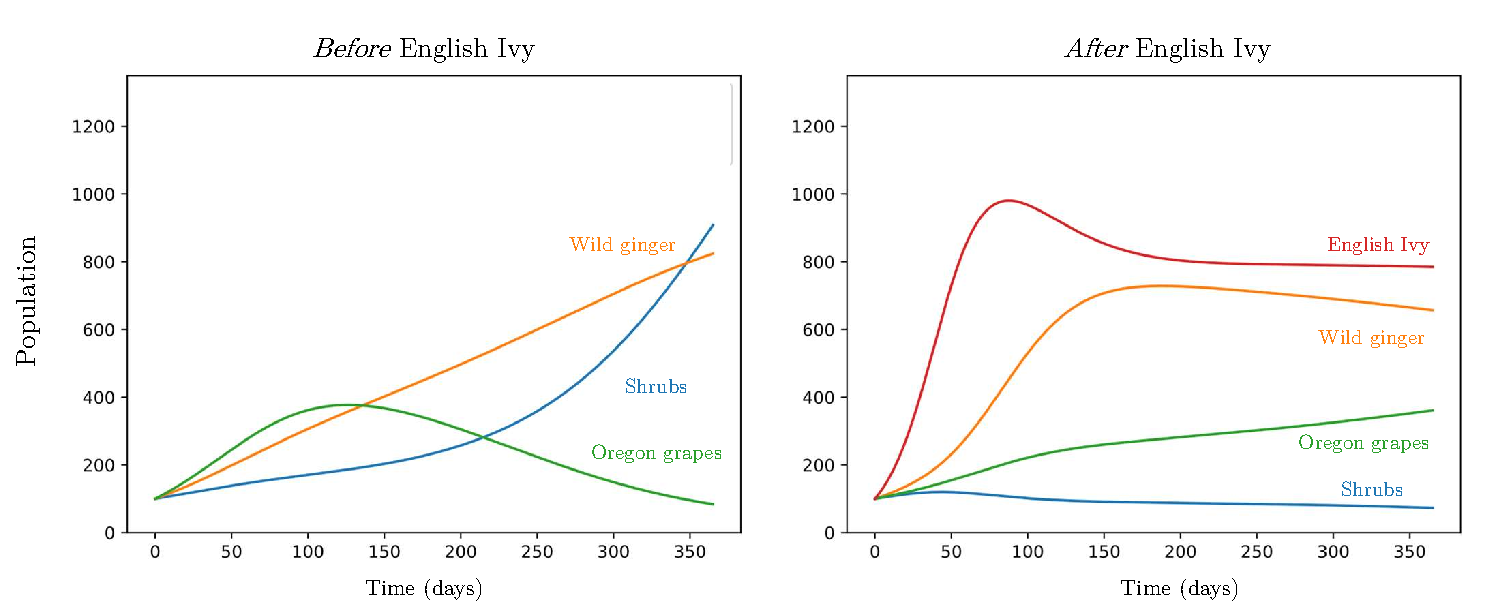
\includegraphics[scale=0.5]{figures/lotkavolterraenglishivy.pdf}
    \captionsetup{width=0.9\textwidth}
    \caption{\textbf{Before and after plot of native species populations of introduction of English ivy species.}}
    \label{fig:lotkavolterraenglishivy}
\end{figure}

From graphing the population solutions to the system, we can see the population shifts in Figure~\ref{fig:lotkavolterraenglishivy}. Based on the numerical solution to this differential equation from scientific computing software, we find the change of populations over a single year (365 days) to be \(\frac{900}{90}\) for shrubs, \(\frac{800}{600}\) for wild ginger, and \(\frac{100}{300}\) for Oregon grapes. So, we can calculate the native species impact score to be

\[\chi = \frac{900}{90} + \frac{800}{600} + \frac{100}{300} = 11.667\]

For the second part of the ecological score, we need to calculate the spreadability index. First, we can start from a commonly regarded fact that English populations can double in around one and a half years in most growing conditions, even in the shade \cite{usdaHederaHelix}. Therefore, by performing logistic regression with the x-axis being days and the y-axis as population, we can find that the \(r\) value is around 0.035. So, our spreadability index can be calculated as \(100r = 3.5\). Therefore, by Equation~\ref{eq:ecologicalimpact}, our ecological impact score is \(3.5 + \chi = 3.5 + 11.667 = 15.167\).

\subsubsection{Economic Potential}
We assume that there exists some small landscaping firm which harvests and grows English ivy plants in a town in Washington, as common landscaping designers use English ivy to decorate their clients' backyards \cite{psuEnglishLandscape}. By analyzing the microeconomic model of this firm, we will be able to calculate our economic profits.

First, we start with estimating the expected marginal cost and revenue of harvesting and growing each pound of English ivy based on the Gordon-Schaefer model. We estimate that the constant marginal cost of harvesting each pound of English ivy is around \(\$15.00\), as in a larger operation, it takes around an hour of manual labor to safely harvest English ivy \cite{bhgCaringEasytoGrow}. 

To estimate marginal revenue, we performed an online survey to estimate revenue per pound of English ivy. Based on several pricing estimates \cite{gardengoodsdirectEnglish}, we conclude that the maximum pricing for a pound of English ivy would fall around \(\$100.00\) and decreasing with slope \(-0.5\) per pound increased of English ivy. After applying the Profit Maximization Law and analyzing this firm like a Gordon-Schaefer model and finding the intersection of the MR and MC curve, it is evident that an optimal English ivy yield would be around 170 lbs for \(\$57.75\) each. 

To calculate economic profits (\(\pi\)), we subtract total costs (\(\$15.00 \cdot 170\)) from total revenue (\(\$57.75 \cdot 170\)), which leads us to conclude that \(\pi = \$7225.00\).

As for measuring social welfare, English ivy has no benefits to humans other than as a landscaping plant, which is already a core part of calculating economic profits. Lastly, for the human risk factor, English ivy is inedible and contains toxic sap, however, there is rarely an incidence where an English ivy plant has harmed a human. Therefore, we deduce that social welfare \(W = 0\) and human risk \(R = 0\). So, our total economic potential can be calculated as 

\[\text{Total Economic Benefit } = \pi + W - R = \$7225.00\]

So, our final invasive species impact score for English ivy plants in Washington is

\[\text{Impact Score} = (\text{Ecological Score, Economic Score}) = (15.167, \$7225.00)\]

\subsection{Score Comparison}

To analyze the differences in each score and the "classification" of each non-native species, we take a look at the trade-offs between ecological and economic scores in our definition of an impact factor.

\begin{table}[h]
\renewcommand{\arraystretch}{1.3}
%p{0.8\linewidth
    \begin{tabularx}{\textwidth}{p{0.21\textwidth}llX}
    \toprule
    \textbf{Non-Native Species}  & \textbf{Ecological} & \textbf{Economic} & \textbf{Analysis} \\ \midrule
    \raggedright Dandelions & 21.794 & \(\$105.46\) & As dandelions have a high ecological impact primarily due to the loss of native populations with a low return in economic potential, we conclude that dandelions are indeed \textit{invasive species}. \\
    \rowcolor{gray!15}
    \raggedright Garlic mustard & 5.278  & \(\$26.00\) & Since garlic mustard plants have a slight ecological impact and have little to none return on economic potential, we label garlic mustard plants as \textit{invasive species.}\\
    \raggedright English ivy & 15.167 & \(\$7225.00\) & As English ivy plants have a high impact on environment yet also have a large return on economic potential, we conclude that English ivy plants \textit{are not invasive}.\\
    \bottomrule
    \end{tabularx}
\end{table}